%-------------------------------------------------------------------------------
% A COGNITIVE SYSTEM
%-------------------------------------------------------------------------------
\subsection{A ``cognitive" system}
\begin{frame}{Introduction}{A ``cognitive" system}


\begin{block}{Problematic}
{
How can FCA  optimise a \textbf{cognitive} memory structure?
}
\end{block}

\vskip7mm

\begin{block}{``Cognition"}
{
  The mental action or process of \textbf{acquiring knowledge} and 
  understanding through \textbf{thought}, \textbf{experience}, and the 
  \textbf{senses}.
}
\vskip2mm
\hspace*\fill{\small--- Oxford Dictionary}
\end{block}

\end{frame}

%-------------------------------------------------------------------------------
% LEARNING FROM EXPERIENCE
%-------------------------------------------------------------------------------
\subsection{Learning from experience}
\begin{frame}{Introduction}{Learning from experience}

Unfamiliar objects are evaluated thanks to familiar attributes\ldots

\vspace{0.5cm}

\begin{figure}[ht]
% KITTEN
\begin{minipage}[b]{0.20\linewidth}
\centering
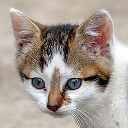
\includegraphics[width=\textwidth]{img/introduction/kitten.png}
\\{\color{green}+100}
\end{minipage}
\hspace{0.1cm}
% SEA URCHIN
\begin{minipage}[b]{0.20\linewidth}
\centering
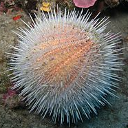
\includegraphics[width=\textwidth]{img/introduction/urchin.png}
\\{\color{red}-100}
\end{minipage}
\hspace{0.1cm}
% KOALA
\begin{minipage}[b]{0.20\linewidth}
\centering
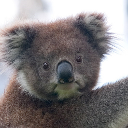
\includegraphics[width=\textwidth]{img/introduction/koala.png}
\\?
\end{minipage}
\hspace{0.1cm}
% ECHIDNA
\begin{minipage}[b]{0.20\linewidth}
\centering
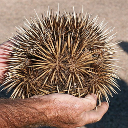
\includegraphics[width=\textwidth]{img/introduction/echidna.png}
\\?
\end{minipage}

\end{figure}
\end{frame}

%-------------------------------------------------------------------------------
% SYTEM LIMITATIONS
%-------------------------------------------------------------------------------
\subsection{System limitations}
\begin{frame}{Introduction}{System limitations}

\ldots{}but beware of certain attribute combinations!

\vspace{0.5cm}

\begin{figure}[ht]
% COFFEE
\begin{minipage}[b]{0.3\linewidth}
\centering
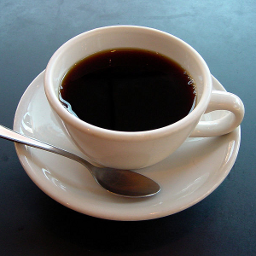
\includegraphics[width=\textwidth]{img/introduction/coffee.png}
\\{\color{green}+100}
\end{minipage}
\hspace{0.5cm}
% LAPTOP
\begin{minipage}[b]{0.3\linewidth}
\centering
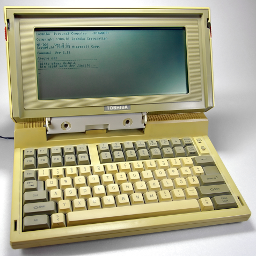
\includegraphics[width=\textwidth]{img/introduction/laptop.png}
\\{\color{green}+100}
\end{minipage}

\end{figure}

\end{frame}

%-------------------------------------------------------------------------------
% HOW FCA CAN HELP
%-------------------------------------------------------------------------------
\subsection{How FCA can help}
\begin{frame}{Introduction}{How FCA can help}

\vspace{0.3cm}

FCA allows for the evaluation of abstract \textbf{concepts}.

\vspace{0.2cm}

\begin{figure}[ht]
\begin{minipage}[b]{0.5\linewidth}
\centering
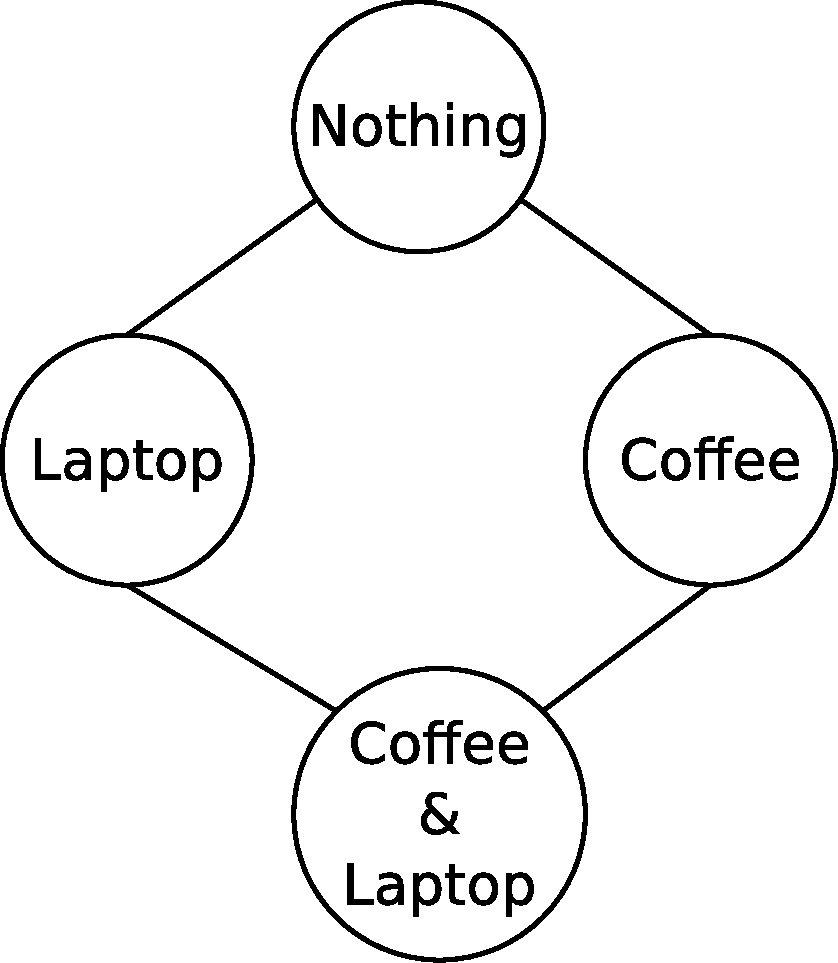
\includegraphics[width=\textwidth]{img/introduction/coffee_laptop.pdf}
\end{minipage}
\end{figure}

\end{frame}